\chapter{Datasety}

Data, s ktorými budeme pracovať, sú výhradne len výsledky a konečné stavy jednotlivých zápasov. 

\section{Futbal} \label{foot}
Pre futbal získame všetky zápasy sezóny pre danú ligu. 
Musia byť všetky, pretože v ďalšej časti sa počíta na základe už odohraných zápasov a jeden zápas by mohol skresliť výsledky. 
Jednotlivé ligy boli teda vyberané nielen na základe kvality, ale aj na základe toho, že v pár posledných sezónach sa ani raz nestalo, že zápas musel byť z nejakého dôvodu udelený kontumačne jednému z tímov (ako sa napríklad stalo vo francúzskej lige v roku 2017 pre problémy s divákmi \citep{awarded}) alebo celá sezóna bola poznačená korupčným škandálom ako v prípade talianskej ligy v sezóne 2006 \citep{scandal}.
Takéto výsledky by nemuseli skresliť stavbu neurónovej siete, ale všeobecne je lepšie, ak sa takýmto situáciám vyhneme.

Dáta pre každú ligu predstavujú výsledky všetkých zápasov odohraných len vrámci ligy za pár posledných sezón. 
Nebudeme používať žiadne dáta informujúce o hráčoch, ktorí sú na oficiálnej súpiske na zápas ani dáta o základnej zostave na daný zápas a ani ďalšie informácie o priebehu zápasu ako percentuálne držanie lopty alebo počet striel, či rohových kopov.
Taktiež vzhľadom na to, že tímy v jednotlivých ligách hrajú zápasy aj mimo ligy, prinajmenšom zápasy v ligovom pohári, nebudú použité ani informácie o oddychu pred daným zápasom, teda koľko dní pred zápasom mali zúčastnené tímy voľno.

Dátaset pre každú ligu je tabuľka, kde riadky predstavujú jednotlivé zápasy zoradené podľa dátumu, v ktorom bol zápas odohraný, zostupne.
Stĺpce sú v poradí:
\begin{enumerate}
  \item Jednoznačný názov domáceho tímu (nemusí byť celý názov, stačí skrátený, ale jednoznačný a, pokiaľ možno, v celom dátasete konzistentný),
  \item Jednoznačný názov hosťujúceho tímu,
  \item Identifikátor zápasu,
  \item Ligové kolo, v ktorom sa zápas odohral (0, ak sa nevie),
  \item Identifikátor domáceho tímu,
  \item Identifikátor hosťujúceho tímu,
  \item Počet gólov strelených domácim tímom v zápase,
  \item Počet gólov strelených hosťujúcim tímom v zápase,
  \item Dátum zápasu,
  \item Sezóna,
  \item Kurz na výhru domácich,
  \item Kurz na remízu,
  \item Kurz na výhru hostí.
\end{enumerate}

Posledné 3 stĺpce teda predstavujú kurzy na dané výsledky. Tieto ale nie sú pri trénovaní siete využívané, a teda pre dáta, ktoré sú vždy použité len pre trénovanie, nie sú nevyhnutné.
\begin{figure} [h!]
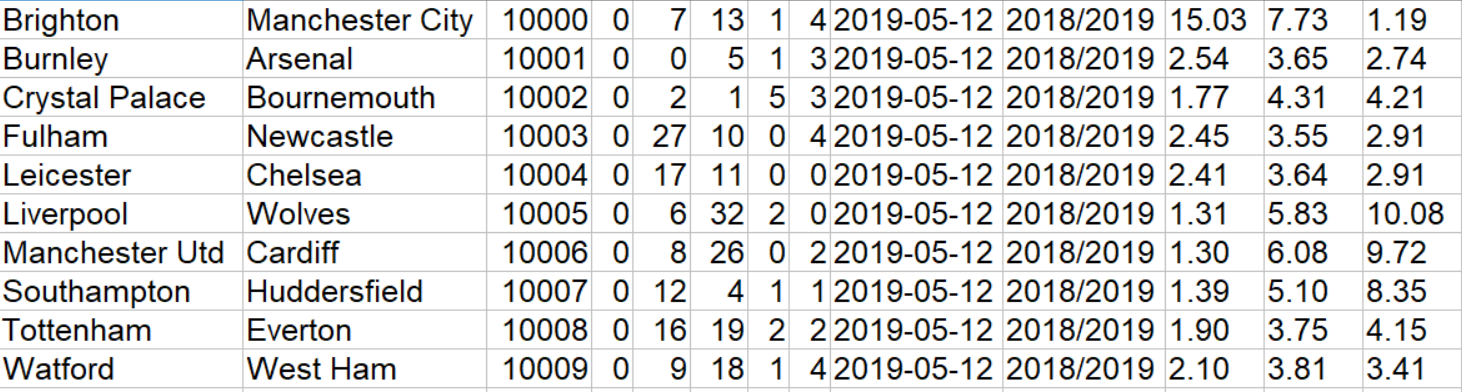
\includegraphics[width=\textwidth]{../img/eng.png}
\caption{Ukážka prvých 10 riadkov z tabuľky všetkých zápasov anglickej Premier League ilustrujúcich členenie tabuľky}
\end{figure}

Dáta v trénovacom súbore obsahujú prvú polovicu sezóny 2018/2019 a 7 jej celých predchádzajúcich sezón. Prvá polovica sezóny predstavuje všetky odohrané zápasy od začiatku sezóny až po odohratie posledného zápasu pred začiatkom kola, ktoré je numericky už v druhej polovici sezóny. 
Napríklad najvyššia anglická futbalová liga, Premier League, má 38 kôl každú sezónu, do úvahy sa bude brať posledných 7 sezón pred sezónou 2018/2019 a všetky zápasy odohrané pred prvým zápasom 20. kola sezóny 2018/2019 (s výnimkou predohrávok, teda zápasov, ktoré boli preložené na dátum pred dátumom, v ktorom daný zápas figuroval v predsezónnom rozpise zápasov).


\subsection{Motivácia pre výber daných príznakov}
Vybrané príznaky presne popísané v sekcii Prílohy (Príloha \ref{in:foot}) sa dajú rozdeliť viacerými spôsobmi do skupín.
Z daných príznakmi sa ešte budú selektovať tie najdôležitejšie v jednej z nasledujúcich sekcii (konkrétne sekcia \ref{stavba}).

Prvým spôsobom je rozdeliť tieto príznaky tak, ako za sebou nasledujú do skupiny po desiatich. To nám vytvorí 5 skupín, môžeme ich po poradí nazvať príznaky sezóny, roly, formy, vzájomných zápasov a doplnkové.

Skupina príznakov sezóny obsahuje dáta o celom doterajšom priebehu sezóny pre obe tímy. Mohlo by byť dôležité vedieť, ako daný tím vystupuje v celej sezóne.

Príznaky roly obsahujú dáta o výsledkoch daných tímov v role, v akej sa predstavia v predikovanom zápase (domáci alebo hostia) počas celej sezóny. To by mohlo byť dôležité, pretože je rozdiel v zápasoch, kde tímy hrajú doma a v zápasoch, kde hrajú vonku. Tento rozdiel je individuálny. Tím môže vyhrávať napríklad len na domácom ihrisku a mimo neho sa im nemusí až tak dariť, v tom prípade by v role hostí nemuseli byť favoritom na víťazstvo, aj keď by to mohla predchádzajúca skupina očakávať.

Tretia skupina je forma.
Hodnotených je posledných 5 zápasov, tradične to v predikovaných ligách predstavuje obdobie 4 -- 5 týždňov.
Forma by mala byť dôležitá, pretože určuje, ako sa tímu darilo v lige v posledných zápasoch, teda predstavuje niečo ako psychickú pohodu tímu, s ktorou vstupuje do zápasu.

Príznaky vzájomných zápasov určujú posledných 5 vzájomných zápasov, ktoré dané tímy odohrali pred predikovaným zápasom. Prvých 5 príznakov sa týka celkových 5 vzájomných zápasov, ďalších 5 sa týka vzájomných zápasov odohraných na ihrisku domáceho v predikovanom zápase. Každý tím hrá iný štýl hry a každý štýl funguje lepšie proti nejakému štýlu a horšie zas proti inému štýlu (to bol jeden z výsledkov vo vyššie spomínanom článku \citep{related:shin}). Tímy svoje štýly nezvyknú meniť veľmi často, pretože obvykle by na to potrebovali aj výmenu hráčov. Cieľom týchto príznakov je ohodnotiť, ako sa obvykle darí daným tímom, keď sa stretnú medzi sebou.

Poslednou skupinou sú zvyšné príznaky určené na trénovanie, a to je dlhodobá sila domáceho a hosťujúceho mužstva a skóre. 
Niekedy sa môže stať, že tím mal ťažký úvod do sezóny, ale z minulých sezón vieme, že sa im v lige darí obvykle oveľa lepšie a môžeme očakávať, že v nasledujúcich zápasoch začnú uhrávať lepšie výsledky. 
To je dôvodom výberu dlhodobej sily mužstva do skupiny príznakov.
Je to najbližšie ako sa môžeme dostať ku abstraktnému ohodnoteniu kvality mužstva, ktoré používali iní autori (ako napríklad Shin a Gasparyan v \citep{related:shin}) z reálnych dát.

Skóre je pokus ohodnotiť formu tímu čo najlepšie jedným údajom.
Čím väčší počet vstupných neurónov, tým viac dimenzií dodávame neurónovej sieti.
S väčším počtom dimenzií rastie objem celkového priestoru, a to znamená, že sa jednotlivé body dát od seba oddeľujú a samotné dáta sa stávajú redšie.
Tomuto fenoménu hovoria vedci kliatba dimenzionality \citep{curse}.
Práve kvôli tomu vznikol pokús vytvoriť umelé príznaky, ktoré by mohli ohodnotiť rozdiel formy oboch tímov v jednom údaji, na rozdiel od desiatich (popísané sú v Prílohe \ref{in:foot} 44 a 45, detailnejšie pod zoznamom).

Každá z prvých 4 skupín obsahuje dvakrát 5 rôznych údajov, z ktorých môžeme opäť spraviť päť skupín príznakov, a to víťazstvá, remízy, prehry, priemerný počet strelených gólov a priemerný počet inkasovaných gólov.

Prvé tri tieto skupiny hovoria samé za seba, snažíme sa predikovať výsledok zápasu, ktorý je buď výhra, remíza alebo prehra z hľadiska oboch tímov. Zvyšné dve skupiny sa snažia z daných dát simulovať niečo ako ofenzívnu a defenzívnu silu mužstva, podobne ako robili iní autori (napríklad \citep{related:igiri}).

\section{Tenis} \label{ten}
Pre tenis získame všetky zápasy každého turnaja ATP typu 500, 1000 a Grand Slam, kde hraá aspoň jeden hráč z Top 100 rebríčka ATP pre danú sezónu.
Dôvodom je fakt, že predikujeme zápasy týchto turnajov medzi hráčmi z Top 100 rebríčka ATP, ale pre týchto hráčov počítame ich momentálnu formu, takže sú pre nás dôležité aj zápasy, ktoré odohrajú proti hráčom, ktorí sa nenachádzajú v Top 100.
Fakt, že množstvo hráčov z Top 100 sa pravidelne zúčastňuje turnajov typu ATP 250, určuje, že niekedy nastúpia dvaja takíto hráči aj proti sebe na takomto turnaji. Vďaka tomu a aj relatívnej kvalite týchto turnajov sme sa rozhodli, že tieto turnaje zoberieme do úvahy (vzájomné zápasy medzi jednotlivými hráčmi na takto ohodnotených turnajoch tiež patria medzi údaje, z ktorých sa stávajú vstupné neuróny (ako vidieť v Prílohe \ref{in:ten})). 

V tenise sa nemôžeme vyhnúť zápasom, ktoré boli nejakým spôsobom udelené jednému z hráčov, či už bez boja alebo po skreči súpera v priebehu zápasu, pretože zranenia sú súčasťou profesionálneho športu.
Vo futbale sa to obvykle rieši prestriedaním zraneného hráča, v tenise to, prirodzene, nie je možné.
Pre potreby tejto práce máme dve možnosti, buď môžeme tieto zápasy úplne ignorovať alebo ich môžeme započítavať do niektorých oblastí vstupu (ako napríklad forma alebo vzájomné zápasy) a ignorovať inde (predpovedať takéto výsledky je možno nápad pre inú prácu). 
Pre potreby tejto práce budeme tieto zápasy úplne ignorovať, čo znamená, že sa nevyskytnú v trénovacích ani testovacích dátach.
Samozrejme, má to svoje výhody aj nevýhody.
Výhodou je, že výsledky budú reálne odzrkadľovať presnosť siete na zápasoch, ktoré sa odohrali a skončili.
Predpovedať zranenie totiž nepatrí medzi ciele tejto práce.
Ďalšou výhodou je spravodlivosť oblastí vstupu ako forma a vzájomné zápasy, pretože sa tam berú len zápasy, ktoré sa dohrali do konca, takže tieto čísla nie sú v žiadnom okamihu nadhodnotené. Ak by napríklad hráč natrafil počas turnaja na dvoch/troch súperov, ktorí sa vzdajú, tak by sa mu vo forme ukázali tieto víťazstvá, aj keď to neboli plnohodnotné výhry.
Nevýhodou je, že výsledky nemusia ukazovať reálne výsledky v praxi (pred zápasom nevieme určiť, či sa hráč zraní, ale sieť aj tak vydá svoju predpoveď, aj keď nebola na tieto údaje trénovaná).

Dátaset je tabuľka, v ktorej každý zápas predstavuje jeden riadok tabuľky, zápasy sú zoradené do turnajov od najskôr odohraných turnajov po tie najbližšie súčasnosti (ak sa obe turnaje začali a končili hrať v rovnaký deň, tak sú v ľubovoľnom poradí, nie je možné, aby poradie zmenilo nejaké dáta, pretože nie je možné hrať na dvoch turnajoch takéhoto typu zároveň). 
Zápasy v turnajoch sú zoradené od finále po prvé kolo, teda intuitívne opačne. Program v transformačnej časti si už to poradie upraví, aby zápasy nasledovali chronologicky. 
Stĺpce tabuľky sú v poradí:
\begin{enumerate}
  \item Názov turnaja,
  \item Počet bodov, ktoré víťaz obrdží za výhru v turnaji (ak to je neznáme, tak je tam nápis N/A)
  \item Rok, v ktorom sa turnaj odohral,
  \item Povrch kurtov na turnaji (tvrdý \textit{(Hard)}, antukový \textit{(Clay)} alebo trávnatý povrch \textit{(Grass)}),
  \item Meno víťaza zápasu,
  \item Meno hráča, ktorý zápas prehral,
  \item Kolo turnaja, v ktorom sa zápas odohral od najdôležitejšieho (1 značí finále, 2 semifinále, apod.),
  \item ID zápasu,
  \item ID víťaza*,
  \item ID porazeného hráča*,
  \item Počet setov, ktoré v zápase získal víťaz,
  \item Počet setov, ktoré v zápase získal porazený hráč,
  \item Počet hier, ktoré v zápase získal víťaz v jednotlivých setoch oddelené znakom |,
  \item Počet hier, ktoré v zápase získal porazený hráč v jednotlivých setoch oddelené znakom |,
  \item Predzápasový kurz na výhru víťaza zápasu,
  \item Predzápasový kurz na výhru porazeného hráča v zápase.
\end{enumerate}
* - ak je ID hráča NULL, znamená to, že hráč sa doposiaľ ani raz neumiestnil v Top 100 rebríčka ATP\\

Postavenia hráčov v rebríčku ATP sú získané z pomocného súboru (ukážku z tohto súboru je možné vidieť na obrázku \ref{rank}), v ktorom sú uchovávané. 
Súbor v transformačnej vrstve práce si pospája hráčov s ich ID a ich umiestnením v práve vyhodnocovanom roku.
\begin{figure} [h!]
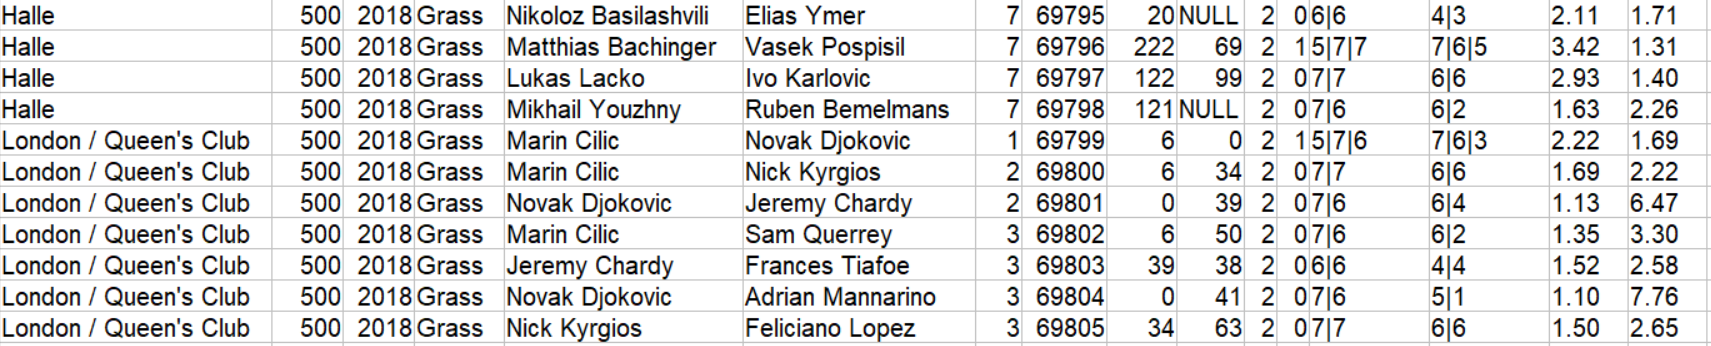
\includegraphics[width=\textwidth]{../img/atp.png}
\caption{Ukážka vybraných pár riadkov z tabuľky zápasov v okruhu ATP ilustrujúcich stĺpce a riadky.}
\end{figure}
\begin{figure} [h!]
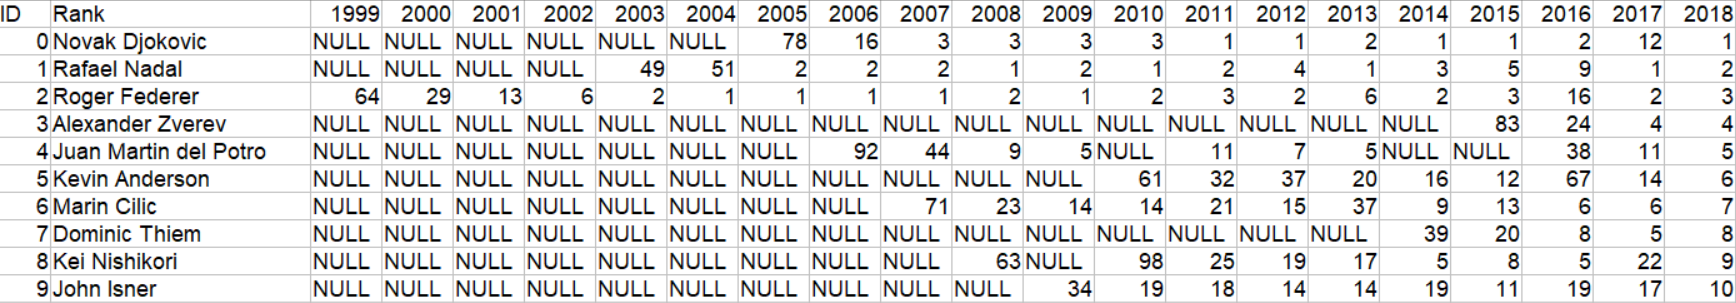
\includegraphics[width=\textwidth]{../img/rank.png}
\caption{Ukážka prvých 10 riadkov spolu aj s hlavičkou z pomocného súboru udržiavajúceho postavenie hráčov v rebríčku ATP. Hodnota \textit{NULL} znamená, že sa hráč na konci daného roku neumiestnil v prvej 100 rebríčka.}
\label{rank}
\end{figure}

\subsection{Motivácia pre výber daných príznakov}
Podobne ako pri futbale si môžeme jednotlivé príznaky zhrnúť do skupín a jednotlivé skupiny predstaviť. Význam jednotlivých príznakov je vypísaný v prílohe (Príloha \ref{in:ten}).

Najprv si môžeme tieto príznaky rozdeliť na skupinové (prvých 30) a jednotlivé.
Na skupinové sa môžeme najprv pozrieť ako na skupiny po 6, a to príznaky roku, formy, povrchu, formy na povrchu a vzájomných zápasov.

Príznaky roku určujú, ako sa danému hráčovi darilo v danom kalendárnom roku.
Táto kategória má zväčša najvyššie hodnoty zo všetkých skupín. Tieto údaje sú dôležitejšie v neskorších fázach roka, pretože ukazujú všeobecný obraz o celom ročníku.

Príznaky formy ukazujú, ako sa hráčovi darilo v posledných 10 zápasoch. Na~rozdiel od futbalu sa tieto dáta prenášajú z roka na rok, takže ak hráč ukončil rok dvakrát po sebe v Top 100 rebríčka ATP počas sledovaných sezón, tak na začiatku druhého roku sa mu ukáže forma aj z minulého roku. Je to tak vyriešené preto, lebo tenis sa hrá v podstate celý rok narozdiel od futbalu, kde liga zvykne končiť v máji a začínať v auguste a počas tejto doby sa môžu udiať zmeny v tíme.
Dôležité sú z podobného dôvodu ako pri futbale, ukazujú momentálnu výkonnosť a psychickú pohodu hráča, s ktorou prišiel do zápasu.

Príznaky povrchu ukazujú, ako hral hráč na povrchu, na ktorom odohrá pre\-di\-ko\-va\-ný zápas, počas roka. V tenise majú rôzne povrchy rôzne vlastnosti. Každý hráč má svoj preferovaný povrch, kde sa mu hrá najlepšie alebo dosahuje najlepšie výsledky. Tieto príznaky ukazujú celkovú výkonnosť daného hráča na tomto povrchu v doterajšom priebehu sezóny.

Príznaky formy na povrchu predstavujú kombináciu oboch predošlých skupín, formy a povrchu. Uchováva údaje o posledných 10 zápasov odohraných na danom povrchu, dáta sa prenášajú cez rok. Dôvody sú dva: prvým je, že obvykle sa rok začína a aj končí na tvrdom povrchu a druhým dôvodom je psychika hráča. Aj keď hráč nehral skoro celý rok na danom povrchu, jeho podvedomie si určite pamätá, ako sa mu tam darilo naposledy, aj na základe toho sa môže tešiť alebo netešiť na zápasy na danom povrchu.

Poslednú skupinu v tomto pohľade predstavujú príznaky vzájomných zápasov, tie sa ešte delia na dve skupiny, všetky vzájomné zápasy a vzájomné zápasy odohrané na povrchu, na ktorom sa bude hrať predikovaný zápas. 
Tieto príznaky by mohli patriť medzi tie najdôležitejšie, ak majú hráči dostatočnú históriu vzájomných zápasov.
Každý hráč má vlastný štýl a proti niektorým štýlom sa mu hrá lepšie ako proti iným. Naviac, narozdiel od futbalu, tenisti za celú svoju kariéru nezvyknú radikálne meniť svoje štýly hry, takže tieto údaje môžu byť relevantné aj po rokoch.
Tieto údaje sú uvedené z pohľadu hráča 1.

Každá táto skupina má údaje o hráčovi 1 a hráčovi 2 v zápase a obsahuje 3 údaje pre každého hráča: počet výhier, prehier a priemerný rozdiel v počte vyhraných a prehraných hier za set. Prítomnosť prvých dvoch je zjavná, snažíme sa predikovať buď výhru alebo prehru. 
Prítomnosť poslednej je tu ako pokus o ukážku sily hráča. 
Táto skupina je postavená na teórii, že sa môže stať, že hráč narážal počas turnaja na hráčov, s ktorými v zápase vyhrával jednoznačne a potom prišiel zápas, kde prehral, ale bol to vyrovnaný zápas. 
Takýto hráč sa potom môže stretnúť s hráčom, ktorý má podobné výsledky, ale ak vyhral, tak to bol tesný zápas a ak prehral, tak prehral jednoznačne.
Pri predikcii výsledku tohto zápasu by bol pravdepodobne favorizovaný prvý hráč, ale ak by sme tento údaj nemali a ostatné údaje by boli dostatočne podobné, tak by mohla mať sieť problémy s rozhodovaním.

Do kategórie jednotlivých príznakov patria umiestnenia oboch hráčov v poslednom koncoročnom rebríčku ATP, kategorizácia povrchu a skóre.
Postavenie hráča v poslednom koncoročnom rebríčku ATP ukazuje, ako sa darilo hráčovi v poslednom roku (keďže rebríček uchováva body z posledného roka). Na tento údaj sa môžeme odvolávať hlavne na začiatku ročníka, keď je ešte málo údajov z tohto roka.

Kategorizácia povrchu je skupina príznakov, ktorá je prítomná hlavne z dôvodu, že pre rôzne povrchy môže fungovať iné ohodnotenie. Napríklad na tvrdom povrchu by sa kládol dôraz na iné aspekty ako na trávnatom povrchu.

Skóre je pokus ohodnotiť formu hráča výraznejšie ako len počtom výhier a prehier. Pri pokusoch a vylaďovaní siete budeme v kapitole Stavba siete (kapitola \ref{stavba}) selektovať dané vstupné neuróny podľa rôznych kritérií a vyskúšame tiež aj ako sa bude sieť správať, ak nahradíme všetky stĺpce obsahujúce dáta o forme rozdielom v skóre.
Teoreticky by sme tým mohli ušetriť 4 vstupné neuróny (forma obsahuje 6 príznakov, ale skóre sa delí na dva príznaky, obe presne popísané v Prílohe \ref{in:ten}).